\chapter{Processamento de Imagens}

O processamento digital de imagens é um campo cujas aplicações são bastante extensas. Existem métodos de processamento de imagens para interesses muito diferentes, que vão desde a melhoria das informações visuais para a interpretação dos médicos até a computação dos dados da imagem para transmissão, armazenamento ou interpretação autônoma por computador \cite{gonzalez}.

O processamento digital de imagens médicas é uma área em grande evolução e uma das que mais representa desafios dentro do processamento de imagens. Mas apesar de ser objeto de pesquisas de várias instituições ao redor do mundo, são poucos os sistemas deste tipo utilizados na prática médica. O principal fator é que este tipo de sistema exige alta eficiência, pois deve ser rápido, para que o tempo de resposta ao paciente não seja grande e ter uma baixíssima taxa de erros. Seus resultados são utilizados para tomar decisões em termos de diagnóstico e escolha de tratamento, por isso, alguns tipos de erro são inadmissíveis.

Em geral, os sistemas de processamento de imagens médicas extraem informações que podem ser provenientes de diversos tipos de modalidades de imagens, como Radiografia, Ultra-sonografia e Ressonância Magnética Nuclear, entre outras. Além das técnicas de processamento de imagens, técnicas de inteligência artificial, reconhecimento de padrões, entre outras áreas computacionais, são também aplicadas com o objetivo de melhorar tais imagens e extrair delas informações úteis ao diagnóstico.

\section{Imagens de tomografia computadorizada}

A tomografia era um dos mais importantes métodos de diagnóstico radiológico até a invenção da tomografia computadorizada, na década de 70 do século passado. Sendo um dos primeiros tipos de exame a se beneficiar da popularização da computação.

A utilização de imagens no campo da medicina tem como principal objetivo proporcionar uma avaliação não invasiva dos tecidos e órgãos do corpo humano, tornando possível a verificação de anormalidades causadas por doenças ou acidentes \cite{oliveira}.

As máquinas de tomografia computadorizada possuem uma fonte de raios x e detectores de raios x, os quais ficam em lados opostos um do outro. Para construir as imagens de tomografia computadorizada a fonte e os detectores de raios x são movidos para posições pre-determinadas e então obtem diversas imagens, como demonstrado \ref{fig:tc1}, as quais representam fatias finas do paciente.

\begin{figure}[ht]
 \begin{center}
  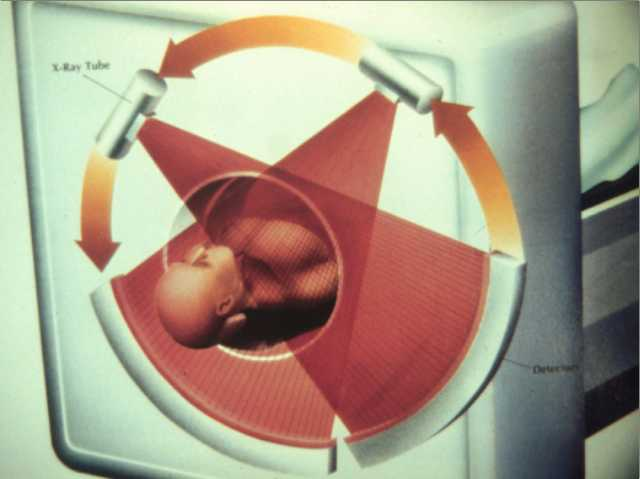
\includegraphics{imagens/tc.jpg}
 \end{center}
 \caption{Demonstração de como uma máquina de tomografia computadorizada obtem as fatias de imagem do paciente.}
% TODO: referencia = http://www.sprawls.org/resources/CTIMG/classroom.htm
 \label{fig:tc1}
\end{figure}

A forma de movimentação depende da tecnologia da máquina utilizada. Nas máquinas mais antigas, eram tiradas várias fotos de uma fatia do paciente, apenas circulando em torno dele, e então depois a "cama" onde o paciente deita-se se move, para outra rodada de fotos, como em \ref{fig:tc2}. Hoje em dia, temos as máquinas helicoidais, os quais descrevem uma hélice em torno do paciente, em vez de uma sucessão de círculos completo. Desta forma é obtida informação de uma forma contínua.

\begin{figure}[ht]
 \begin{center}
  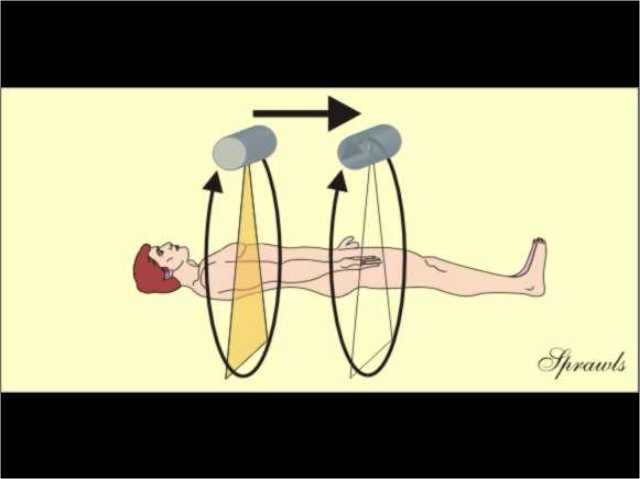
\includegraphics{imagens/tc2.jpg}
 \end{center}
 \caption{Forma de movimentação de máquinas de TC de tecnologia antiga.}
% TODO: referencia = http://www.sprawls.org/resources/CTIMG/classroom.htm
 \label{fig:tc2}
\end{figure}

O resultado de cada pixel das fatias obtidas é a soma das energias bloqueadas pelos tecidos do corpo, e sabe-se exatamente em que ângulo cada fatia foi tirada, por isso após a aquisição das seções transversais, é possivel a reconstrução da imagem em até 3 dimensões. Para a reconstrução é utilizada uma técnica matemática chamada de projeção retrógrada, ou outras, como a transformada de Fourier.

% expandir ou nao expandir? eis a questão.

Essas imagens são geralmente de 512x512 pixels, embora alguns equipamentos possuam uma resolução de 1024x1024 pixels. O tamanho do pixel é da ordem de 1mm, podendo chegar em algumas unidades a valores em torno de 0,1mm.
% referencia

\subsection{Coeficiente de Hounsfield}

A escala da unidade hounsfield é uma transformação linear da medida do coeficiente de atenuação linear original, do qual a radiodensidade da água destilada a temperatura e pressão ambientes é definida como 0 unidades Hounsfield, enquanto a radiodensidade do ar a temperatura e pressão ambientes é -1000 unidades Hounsfield. Para um material X com coeficiente de atenuação $\mu$X, o correspondente valor em unidades Hounsfiled é dado por \ref{equa:hounsfield}.

\begin{equation}
	\frac{\mu_X-\mu_{H_2O}}{\mu_{H_2O}-\mu_{ar}}\times 1000
	\label{equa:hounsfield}
\end{equation}

onde $\mu_{H_2O}$ e $\mu_{ar}$ são os coeficientes de atenuação linear da água e do ar, respectivamente, a pressão e temperatura ambientes. Então uma mudança de uma unidade Hounsfield representa uma mudança de 0,1\% da diferença do coeficiente de atenuação entre a água e o ar, ou aproximadamente 0,1\% do coeficiente de atenuação da água, já que o coeficiente de atenuação do ar é aproximadamente 0. Alguns valores Hounsfield conhecidos estão mostrados na \ref{tab:hounsfield}.

\begin{table}
 \label{tab:hounsfield}
 \caption{Valores Hounsfield comuns.}
 \cite{oliveira} % TODO: funciona?
 \begin{center}
 \begin{tabular}{|l|r|}
 \hline
%TODO: trocar palavra tecido
 	\textbf{Tecido} & \textbf{Unidade Hounsfield} \\ \hline
 	Ar & -1000 \\ \hline
 	Pulmão & -900 a -400 \\ \hline
 	Gordura & -110 a -65 \\ \hline
 	Água & 0 \\ \hline
 	Rim & 35 \\ \hline
 	Sangue normal & 35 a 55 \\ \hline
 	Sangue coagulado & 80 \\ \hline
 	Músculo & 40 a 60 \\ \hline
 	Fígado & 50 a 85 \\ \hline
 	Ossos & 130 a 250 \\
 \hline
 \end{tabular}
 \end{center}
\end{table}

\subsection{Técnica de Janelas}

O olho humano tem a capacidade de diferenciar uma escala de cinzas de 10 a 60 tons (a maioria das pessoas distingue 20 diferentes tons), enquanto na tomografia há no mínimo 2000 tons. A técnica de janelas é na verdade uma forma de mostrar apenas uma faixa de tons de cinza que nos interessa, de forma a adaptar a nossa capacidade de visão aos dados obtidos pelo tomógrafo.
%TODO: referencia

Precisamos definir os valores máximo e mínimo da janela, para mapear os valores em unidades Hounsfield em níveis de cinza. Todos os valores abaixo do valor mínimo serão mapeados como preto e todos acima do máximo como branco. Para definir estes valores, especificamos o tamanho da janela em unidades Hounsfield e o centro dela, como podemos ver em \ref{fig:tc_janela}.

\begin{figure}[ht]
 \begin{center}
  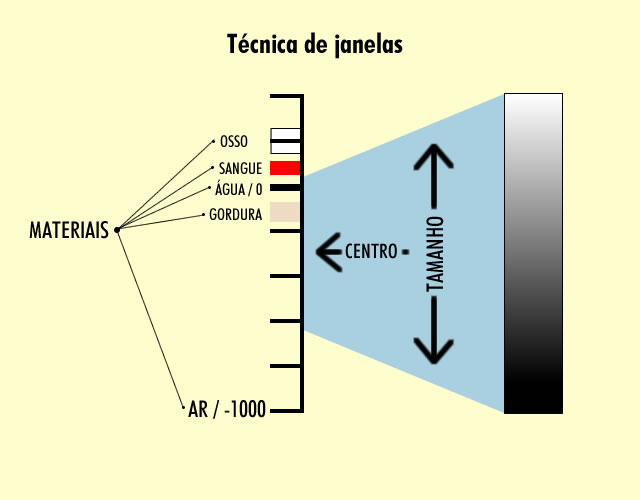
\includegraphics[height=3.0in]{imagens/tc_janela.jpg}
 \end{center}
 \caption{Exemplo de janela.}
%TODO: finalizar
 \label{fig:tc_janela}
\end{figure}

O uso de diferentes janelas em tomografia permite por exemplo o estudo dos ossos com distinção entre a cortical e a medular óssea ou o estudo de partes moles com a distinção, por exemplo, no cérebro entre a substância branca e a cinzenta. A mesma imagem pode ser mostrada com diferentes ajustes da janela, de modo a mostrar diferentes estruturas de cada vez. Não é possível usar um só ajuste da janela para ver, por exemplo, detalhes ósseos e de tecido adiposo ao mesmo tempo. Alguns valores comuns de janela estão na \ref{tab:janela}.

\begin{table}
 \label{tab:janela}
 \caption{Valores comuns de janela para certos tipos de exame.}
% TODO: referencia
% TODO: fazer tabela
 \begin{center}
 \begin{tabular}{|l|r|r|}
 \hline
 	\textbf{Exame} & \textbf{Largura da janela} & \textbf{Centro da janela} \\ \hline
 	Ar & -1000 \\ \hline
 	Pulmão & -900 a -400 \\ \hline
 	Gordura & -110 a -65 \\
 \hline
 \end{tabular}
 \end{center}
\end{table}

\subsection{Artefatos}

% imperfeições da máquina - artefatos

\subsection{Padrão DICOM}

A introdução de imagens médicas digitais na década de 70 do século passado e o uso de computadores para processar estas imagens fizeram com que o American College of Radiology (ACR) e a National Electrical Manufacturers Association (NEMA) se juntassem para formar um comitê com o objetivo de criar um método padrão para a transmissão de imagens médicas e das informações associadas a elas.

Este comitê, constituído em 1983, publicou seu primeiro conjunto de padrões, chamado de ACR-NEMA, em 1985, e o segundo em 1988. Até a publicação dos padrões, a maioria dos equipamentos utilizava formatos proprietários para fazer o armazenamento e comunicação de imagens.

Embora as primeiras versões não tenham obtido êxito total na definição de um padrão comum, a terceira versão, publicada em 1993 sob o nome de DICOM (Digital Imaging and Communications in Medicine), conseguiu estabelecer uma forma padronizada de armazenamento e comunicação de imagens médicas e as correspondentes informações associadas.

Com os melhoramentos promulgados por esta terceira versão, o padrão estava pronto tanto para permitir transferência de imagens médicas em um ambiente com múltiplos fabricantes como também para facilitar o desenvolvimento e a expansão dos sistemas de armazenamento e de comunicação e a conexão com os sistemas de informação médica \cite{nema}.

Nos dias de hoje, a maioria dos fabricantes de equipamentos para aquisição de imagens médicas permite que os arquivos sejam exportados nesse formato, além dos formatos proprietários. Assim como a maioria dos softwares de processamento de imagens médicas também apresenta compatibilidade com esse formato.

\section{Segmentação}

Segmentação é a área do processamento de imagens que trata de isolar as regiões de interesse de uma imagem ou mudar a sua representação para facilitar a sua análise em determinada aplicação. Segmentação de imagens é tipicamente usada para localizar objetos e formas (curvas, linhas, etc) em imagens.

A segmentação de imagens não triviais é uma das tarefas mais difíceis no processamento de imagens. A precisão da segmentação determina o sucesso ou falha de um sistema de análise computadorizada \cite{gonzalez}.

Mas o processo de segmentação é enormemente facilitado quando o domínio das imagens do problema é bem conhecido e restrito. Desse forma permitindo que as técnicas de segmentação possam ser alteradas para trazer resultados mais satisfatórios no domínio do problema.

\subsection{Threshold Adaptativo}

Threshold é um dos métodos mais simples de segmentação de imagens. A partir de uma imagem em tons de cinza, o threshold pode ser usado para torná-la binária.

Durante o processo de threshold, os pixels são dividos em dois grupos, na forma mais simples de threshold, a divisão é feita dependendo apenas se o valor do pixel é maior ou menor que o valor de threshold. Então um grupo é colorido de preto e o outro de branco, tornando a imagem binária. A divisão dos grupos de pixels pode ser feita com base em mais de um valor de threshold, dessa forma os pixels são divididos entre os que estão dentro de um intervalo formado por 2 valores de threshold e os que não estão.

O parâmetro chave que determina a eficiência de um threshold é o valor de threshold usado. Diversos métodos existem para a escolha do valor de threshold, ele pode ser escolhido manualmente, ou por algum algoritmo que o compute, dependendo da imagem, esse tipo de threshold mais conhecido como thresolhd automático. Um método simples é escolher o valor da media ou da mediana. Geralmente esse algoritmo só irá atingir bons resultados se a imagem de entrada possuir pouco ruído e for uniforme. Uma abordagem um pouco mais sofisticada seria gerar o histograma da intensidade dos pixels da imagem e escolher como threshold o valor de vale.

A técnica de threshold adaptivo, que pode ser vista em \ref{fig:threshold}, consiste em escolher um valor inicial arbitrário de threshold ($T^0$), realizar o threshold e calcular o valor médio dos pixels acima ($\mu_{acima}$) e abaixo ($\mu_{abaixo}$) do valor de threshold. Então obter um novo threshold ($T^{i+1}$), de acordo com \ref{equa:thresholdAdaptativo}. Com o novo threshold o processo se inicia novamente, e só para quando atingir a convergência, ou seja, o novo valor for igual ao antigo valor ($T^i = T^{i+1}$). Este algoritmo garante a convergência até um mínimo local.

\begin{equation}
 T^{i+1} = \frac{\mu_{acima}+\mu_{abaixo}}{2}
 \label{equa:thresholdAdaptativo}
\end{equation}

\begin{figure}[ht]
 \begin{center}
  \subfigure[Imagem original]{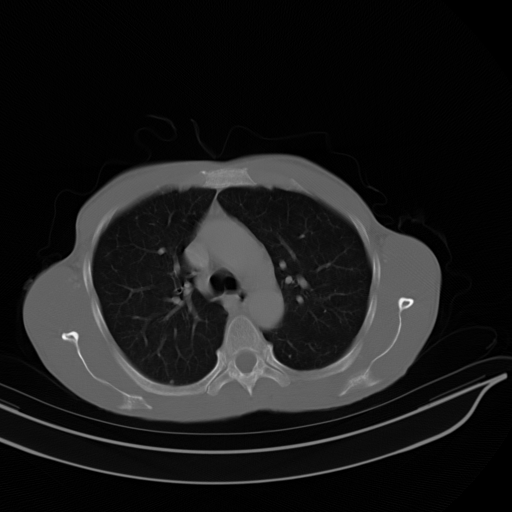
\includegraphics[width=2.5in]{imagens/TCpulmao.png}}
  \subfigure[Depois do threshold adaptativo]{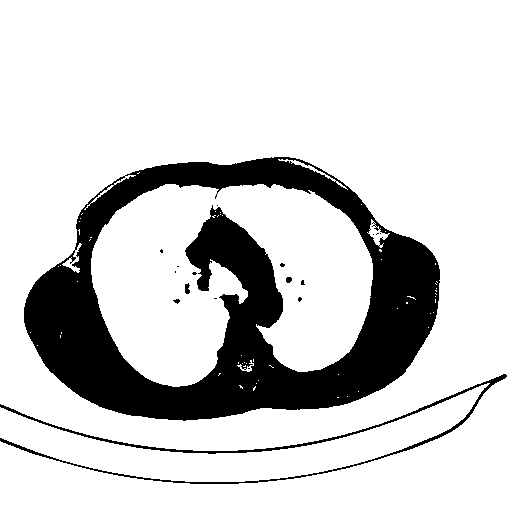
\includegraphics[width=2.5in]{imagens/TCpulmaoTHRESHOLDED.png}}
 \end{center}
 \caption{Imagem de tomografia computadorizada original e após a aplicação de threshold adaptativo.}
 \label{fig:threshold}
\end{figure}

\section{Morfologia Matemática}

Morfologia é o estudo da forma. Em processamento de imagens, morfologia matemática é o nome que se dá a um conjunto de métodos, inicialmente desenvolvidos por Georges Matheron e Jean Serra  em 1964, que têm em comum o objetivo de estudar a estrutura geométrica de uma imagem.

A linguagem utilizada na morfologia matemática é a teoria dos conjuntos. Conjuntos na morfologia matemática representam objetos numa imagem. Por exemplo, o conjunto de todos os pixels pretos numa imagem binária é uma descrição morfologica completa da image. Em imagens binárias, os conjuntos em questão são membros do espaço dos inteiros em duas dimensões $Z^2$, onde cada elemento do conjunto é uma tupla cujas coordenadas são as coordenadas de um pixel preto na image. Imagens em tons de cinza podem ser representadas como conjuntos cujos componentes estão em $Z^3$. Neste caso, dois componentes de cada elemento do conjunto se referem as coordenadas do pixel, e o terceiro corresponde ao valor do seu nível de cinza. Conjuntos em espaços dimensionais ainda mais elevados podem conter outros atributos da imagem, como cor ou componentes que variam com o tempo \cite{gonzalez}.

As operações fundamentais da morfologia matemática são a erosão e a dilatação. Essas operações necessitam do que chamamos de elementos estruturantes. Estes elementos, tão simples quanto matrizes, determinam quais pixels da imagem são retirados (no caso de uma erosão) ou quais são adicionados (no caso de uma dilatação) aos objetos.

%TODO: continua

%TODO: matriz do elemento estruturante
%TODO: exemplo de antes de depois do erosão+dilatação

\section{Extração de características}

\subsection{Histograma}

\subsection{Matriz de co-ocorrência}

\subsection{Características de Haralick}